\chapter{Design}
\label{chap:Design}
In this chapter I will look into designing the system, starting out with how the
database should look in order for it to be able to store the data in a way that
allows me to easily access it again, while reducing redundant data stored. 

After the database I will get into how the system will be structured, which
includes explaining the model that I will be following. After this I will give a
short explanation of some of the patterns I will be following, and why they are
useful for a system such as this one. In the end I will talk about the class
diagrams describing the system.

\section{Database}
\label{sec:Database}
The design of the database will look similar to the domain model
in figure~\ref{fig:domain_model} on many points. This is because on a lot of the
points in this system the domain model can be saved directly to the database. I
have of course had to make some adjustments, as can be seen in
figure~\ref{fig:er_diagram}.

\begin{figure}
  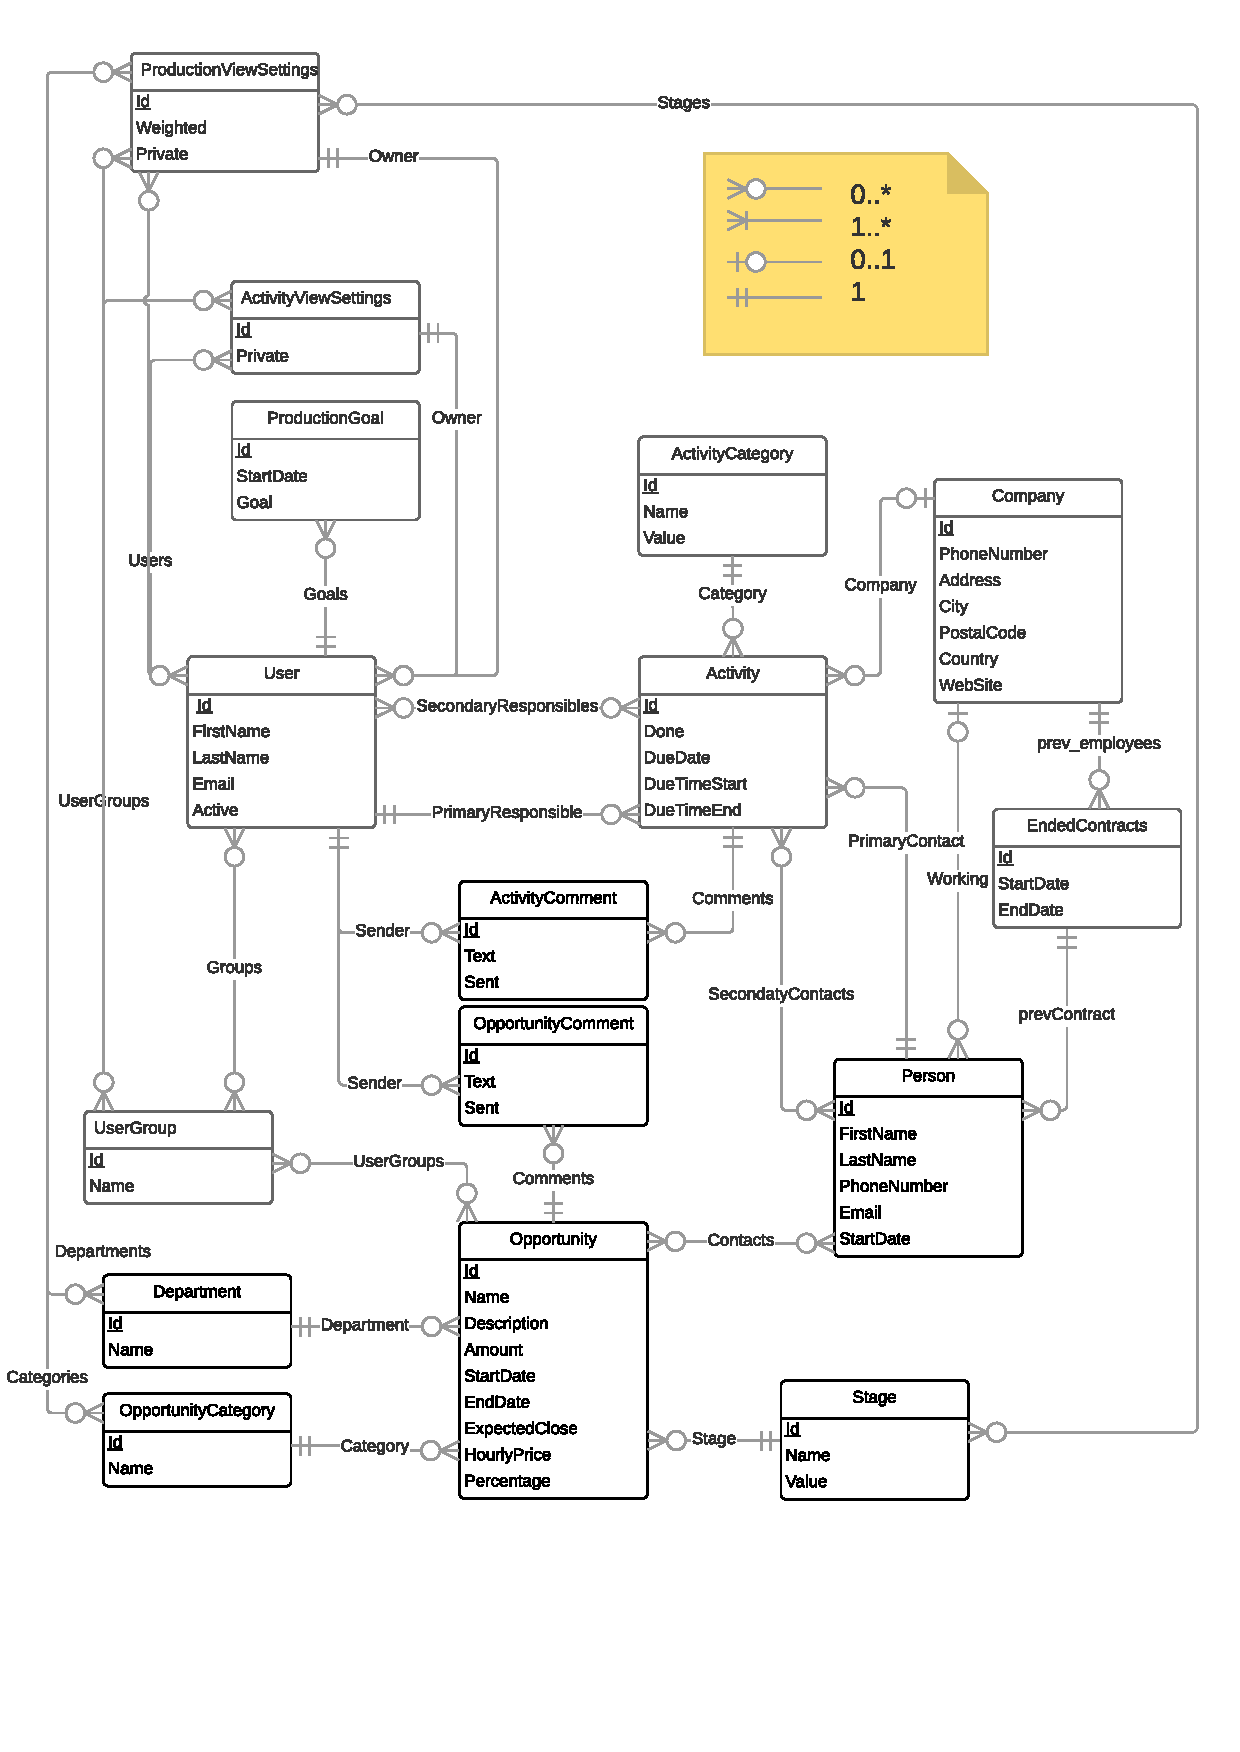
\includegraphics[width=\textwidth]{ER_diagram}
  \caption{ER diagram}
  \label{fig:er_diagram}
\end{figure}

The design is in NF1\footnote{First Normal Form} because I do not have any rows
containing any duplicate information, such as a company having a column for all
their workers, instead the workers are separated out into a different
table\cite[p.~430]{DB_systems}, the same is true for a user and their goals and
user groups, instead of having a list of them in the table itself, I have it
separated out into different tables. 

It is also in NF2\footnote{Second Normal Form} because none of the properties of
any of the tables are functionally dependent on anything other than the primary
key of the table\cite[p.~434]{DB_systems}. 

The next normal form would be the third normal form. I have come to the
conclusion that it is not worth the extra complexity and work of perusing this
last part as the goal with it is to reduce redundant data to even greater
extent, which would mean I would have to move the location based fields of
Company out into a separate table in order for me to remove the transitive
dependency\cite[p.~436]{DB_systems} there is between the city, address, and
postal code, as well as the country. The reason for not pursuing this is that I
have deemed the gain not worth it, since it would bind all locations in the same
area together, and the users may not be interested in this, since if they then
change the postal code or city name of one company, the rest that is located in
the same place will follow. Usually this would be desirable, but since the input
could have been wrong, or a temporary placeholder value depending on how the
users use the system it could cause problems. 

Some people argue that nulls should be allowed and others that there should be
no nulls in a database\cite{stackexchange:db:nullfields}, I do see the reasoning
of both arguments. The argument against null is that generally you cannot know
what null represents, it could mean the absence of data purposefully, or
something else.

One argument is if there is a null value in eg. an integer could mean both zero
and unknown. A solution to avoiding null values in a database could be to split
it into several tables, one for each potential missing value. I have decided not
to do this, since it would make the diagram harder to read, and the database
harder to comprehend. Another reason I have chosen not to get rid of all nulls
is that I have decided that if a value can be and is null. Then it means that
value is not meant to be there. So I will not interpret null as anything but the
absence of data.

As an example if we look at the table Company, the website field is nullable, as
can be seen in the generated database diagram in figure~\ref{fig:database_diagram}.
Here if I have a value of an empty string, it would mean that the website of
the company is known to be non existent. If the field is not set, I know that
the company may have a website, it is just not known in the system.

This forces me to still think about if I should allow a value to be null or not,
without forcing me out of the possibility which is why I have chosen that
solution. 

\doublepagepdf{Schema_diagram}{Database diagram generated with SQL
      Server}{fig:database_diagram} 

\section{System structure}
\label{sec:System structure}
The structure of the system follows the onion
architecture\cite{onion_architecture}, which means that it is build up of layers
as shown in figure~\ref{fig:Onion architecture}. 

\begin{figure}[h]
  \centering
  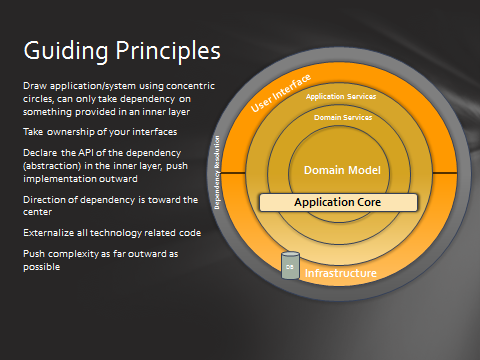
\includegraphics{onion_model}
  \caption[Onion architecture]{Onion architecture\protect\footnotemark}
  \label{fig:Onion architecture}
\end{figure}
\footnotetext{Source: http://www.matthidinger.com/images/www\_matthidinger\_com/Windows-Live-Writer/ff0d136aee1f\_88EA/image\_2.png}

In figure~\ref{fig:structure} the setup that my project will follow is
illustrated. As can be seen I have three core projects, one for each of the core
layers of the model, and outside this I have an infrastructure layer, which is
responsible for talking to the database. The way the outer most layers then work
is by using the interfaces that is defined in \textit{Core.DomainServices}.
These interfaces describe how the application can access the data no matter how it is
stored. 

\begin{figure}[h]
  \centering
  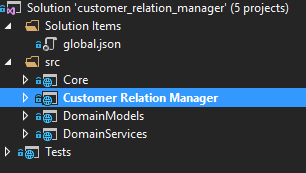
\includegraphics{structure}
  \caption{Structure of the system}
  \label{fig:structure}
\end{figure}

I use injection to allow for easier testing, and lower dependency between the
classes. In the project \textit{customer\_relations\_manager}
which is where the controllers are implemented that clients will be calling, the
controllers take interfaces for the repositories defined in
\textit{Core.DomainServices}. The injection system then is set up to inject the
classes from \textit{Infrastructure.DataAccess} that implement the interfaces. 

The \textit{Core.ApplicationServices} project is there in the case that I need a
service that is not related to accessing data from the data store, but instead
doing something else, such as manipulate data so that it is ready to be plotted
in a graph.

Finally the inner most layer is the classes describing the data that is stored
somewhere, in my case in a database. The name of this project is
\textit{Core.DomainModels}. Their job is to describe how the data looks in the
database, and they are used for making the database first migrations, as well as
make it easy to work with the data in the data store without caring where it is.

The \textit{UnitTests} project is on the same level as
\textit{customer\_relations\_manager}, which means that it is allowed to see
everything in the project, allowing it to test it all. 

The goal with all this separation is to both make it easier to swap out parts of
the project without too much hassle, and to be able to reuse parts, in case I
want to do something similar in the future. It does however also enforce some
order with dependencies, since the domain models are never allowed to know
anything other than them selves, and the data access layer cannot say anything
about how the data will look in the end, only find and filter on it. 

\subsection{Sequences}
\label{subsec:sequences}
To illustrate some of the flows in the system I have made two sequence diagrams,
that go over some standard things the system will do. Namely viewing the goals
of users, in the system, and creation of an opportunity.

The sequences are also tested as integration tests, which will be explained
further in section~\ref{sec:integration_tests}.

For the first sequence diagram i have described how the system works when a user
wants to get the graph data of goals. This can be seen in
figure~\ref{fig:goal_sequence}.

The initial call is a get, which means that the client expects to get some data
back from the server, as that is the primary objective of the call. In the get
the client sends a filter, in this case that could be the time span it is
interested in, and maybe also which users or groups of users they want data for.

The first thing that happens on the server side is that we correct the dates,
since I have decided that if no date is given it means that we return a span of
one year, starting in January of the current year. This also makes sure that if
the user swapped to and from I can still figure out what they meant, as I just
swap them in that case. 

The next step revolves around getting the data from the database, here we apply
the filters, and ask our repository to give all the goals it can find with that
filter. It has a sub call to do the filtering for it, as multiple functions use
the same filtering mechanisms in that class.

When the goals are returned we hand them to the applicationServices, who will
manipulate the data, so that it is in the correct format, and remove unnecessary
information before returning with the data. When the data is returned it is
wrapped, to inform the caller of any changes we may have made to the dates, and
we return an OK with the wrapped data. The OK return is to indicate that it is a
return via the HTTP connection, with a status code of 200.

\begin{figure}[!htbp]
\centering
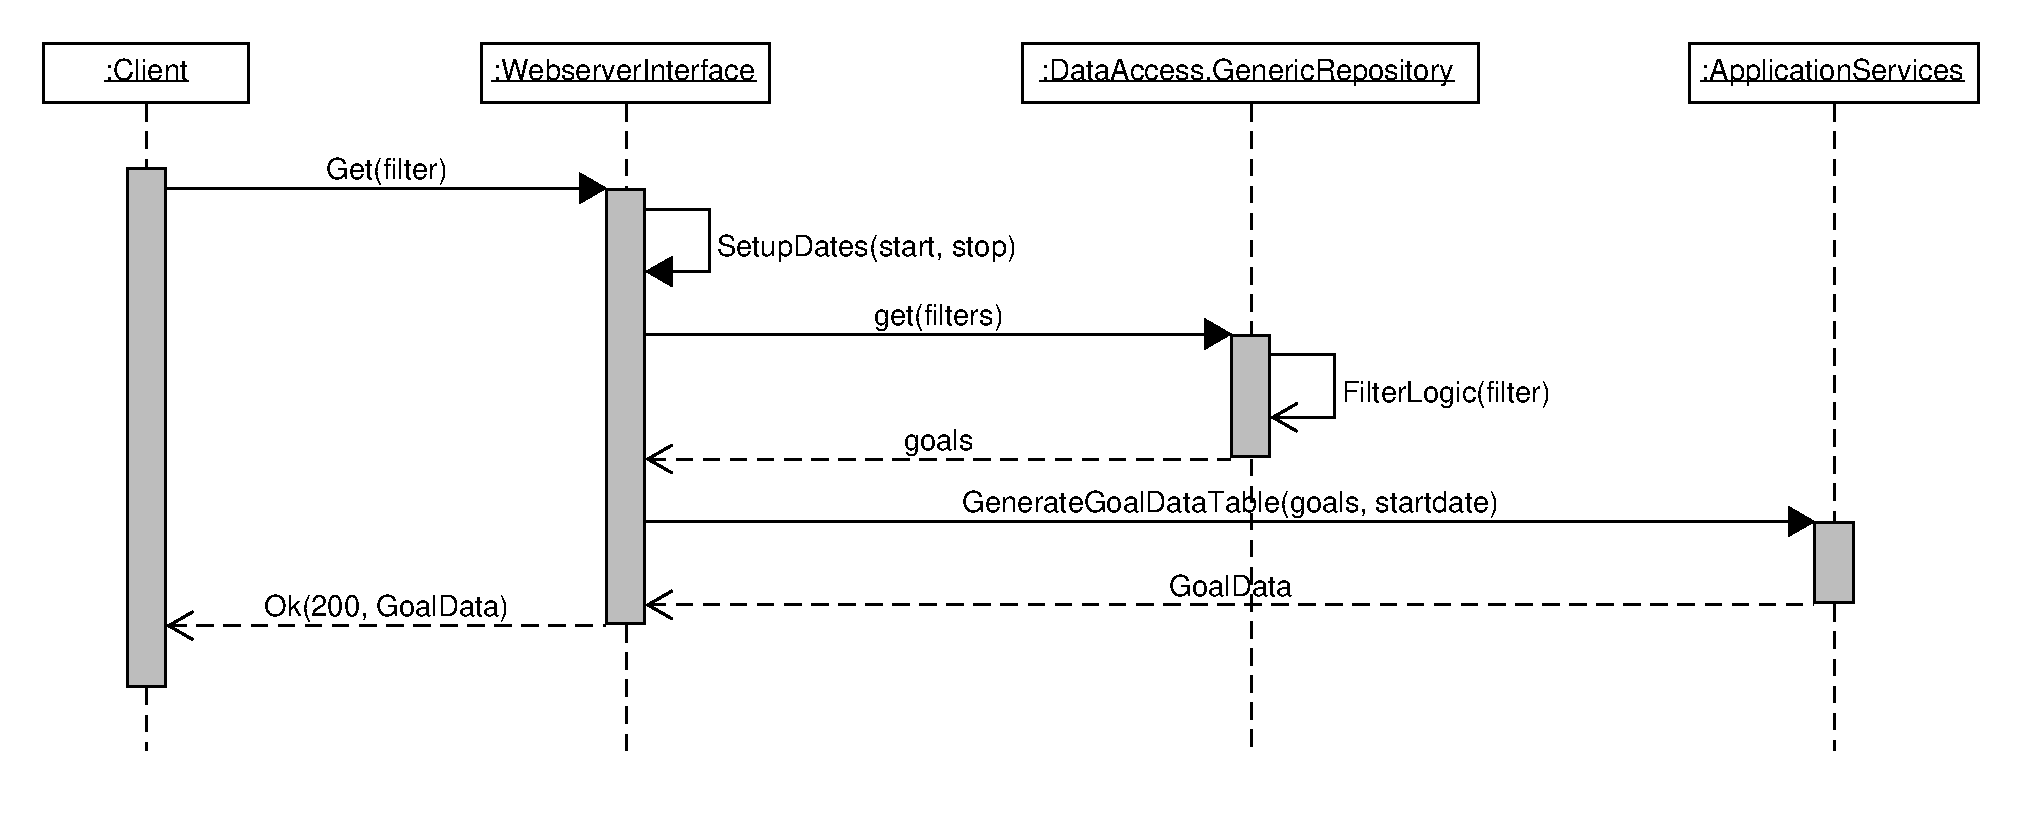
\includegraphics[width=\textwidth]{goal_sequence}
\caption{Sequence diagram for getting data for goals}
\label{fig:goal_sequence}
\end{figure}

For the sequence diagram describing the creation of an opportunity, as can be
seen in figure~\ref{fig:opportunity_sequence} we have start with a Post call the
the server, this post call contains the data that the client wants to create an
opportunity of. Because we cannot assume that the client sends valid data we have
to verify, and if the data is not valid we return BadRequest, which is an HTTP
return type with the code 400, we also tell the client why the request was not
acceptable, as that can help the user fill out missing fields, or correct the
request. 

If the data is okay we ask the repository to create the opportunity. In order
for the repository to verify that all the fields exist, and to link them up it
checks with the database. Some of the fields are optional, as can be seen with
the company and contact, and if they are not set we don't contact the database
about them.

In the end we create the new opportunity in our database layer, and return the
created entity to the interface, that persists the data with save using the Unit
of Work pattern as described in section~\ref{sub:unit_of_work_pattern}.

\begin{figure}[!htb]
  \centering
  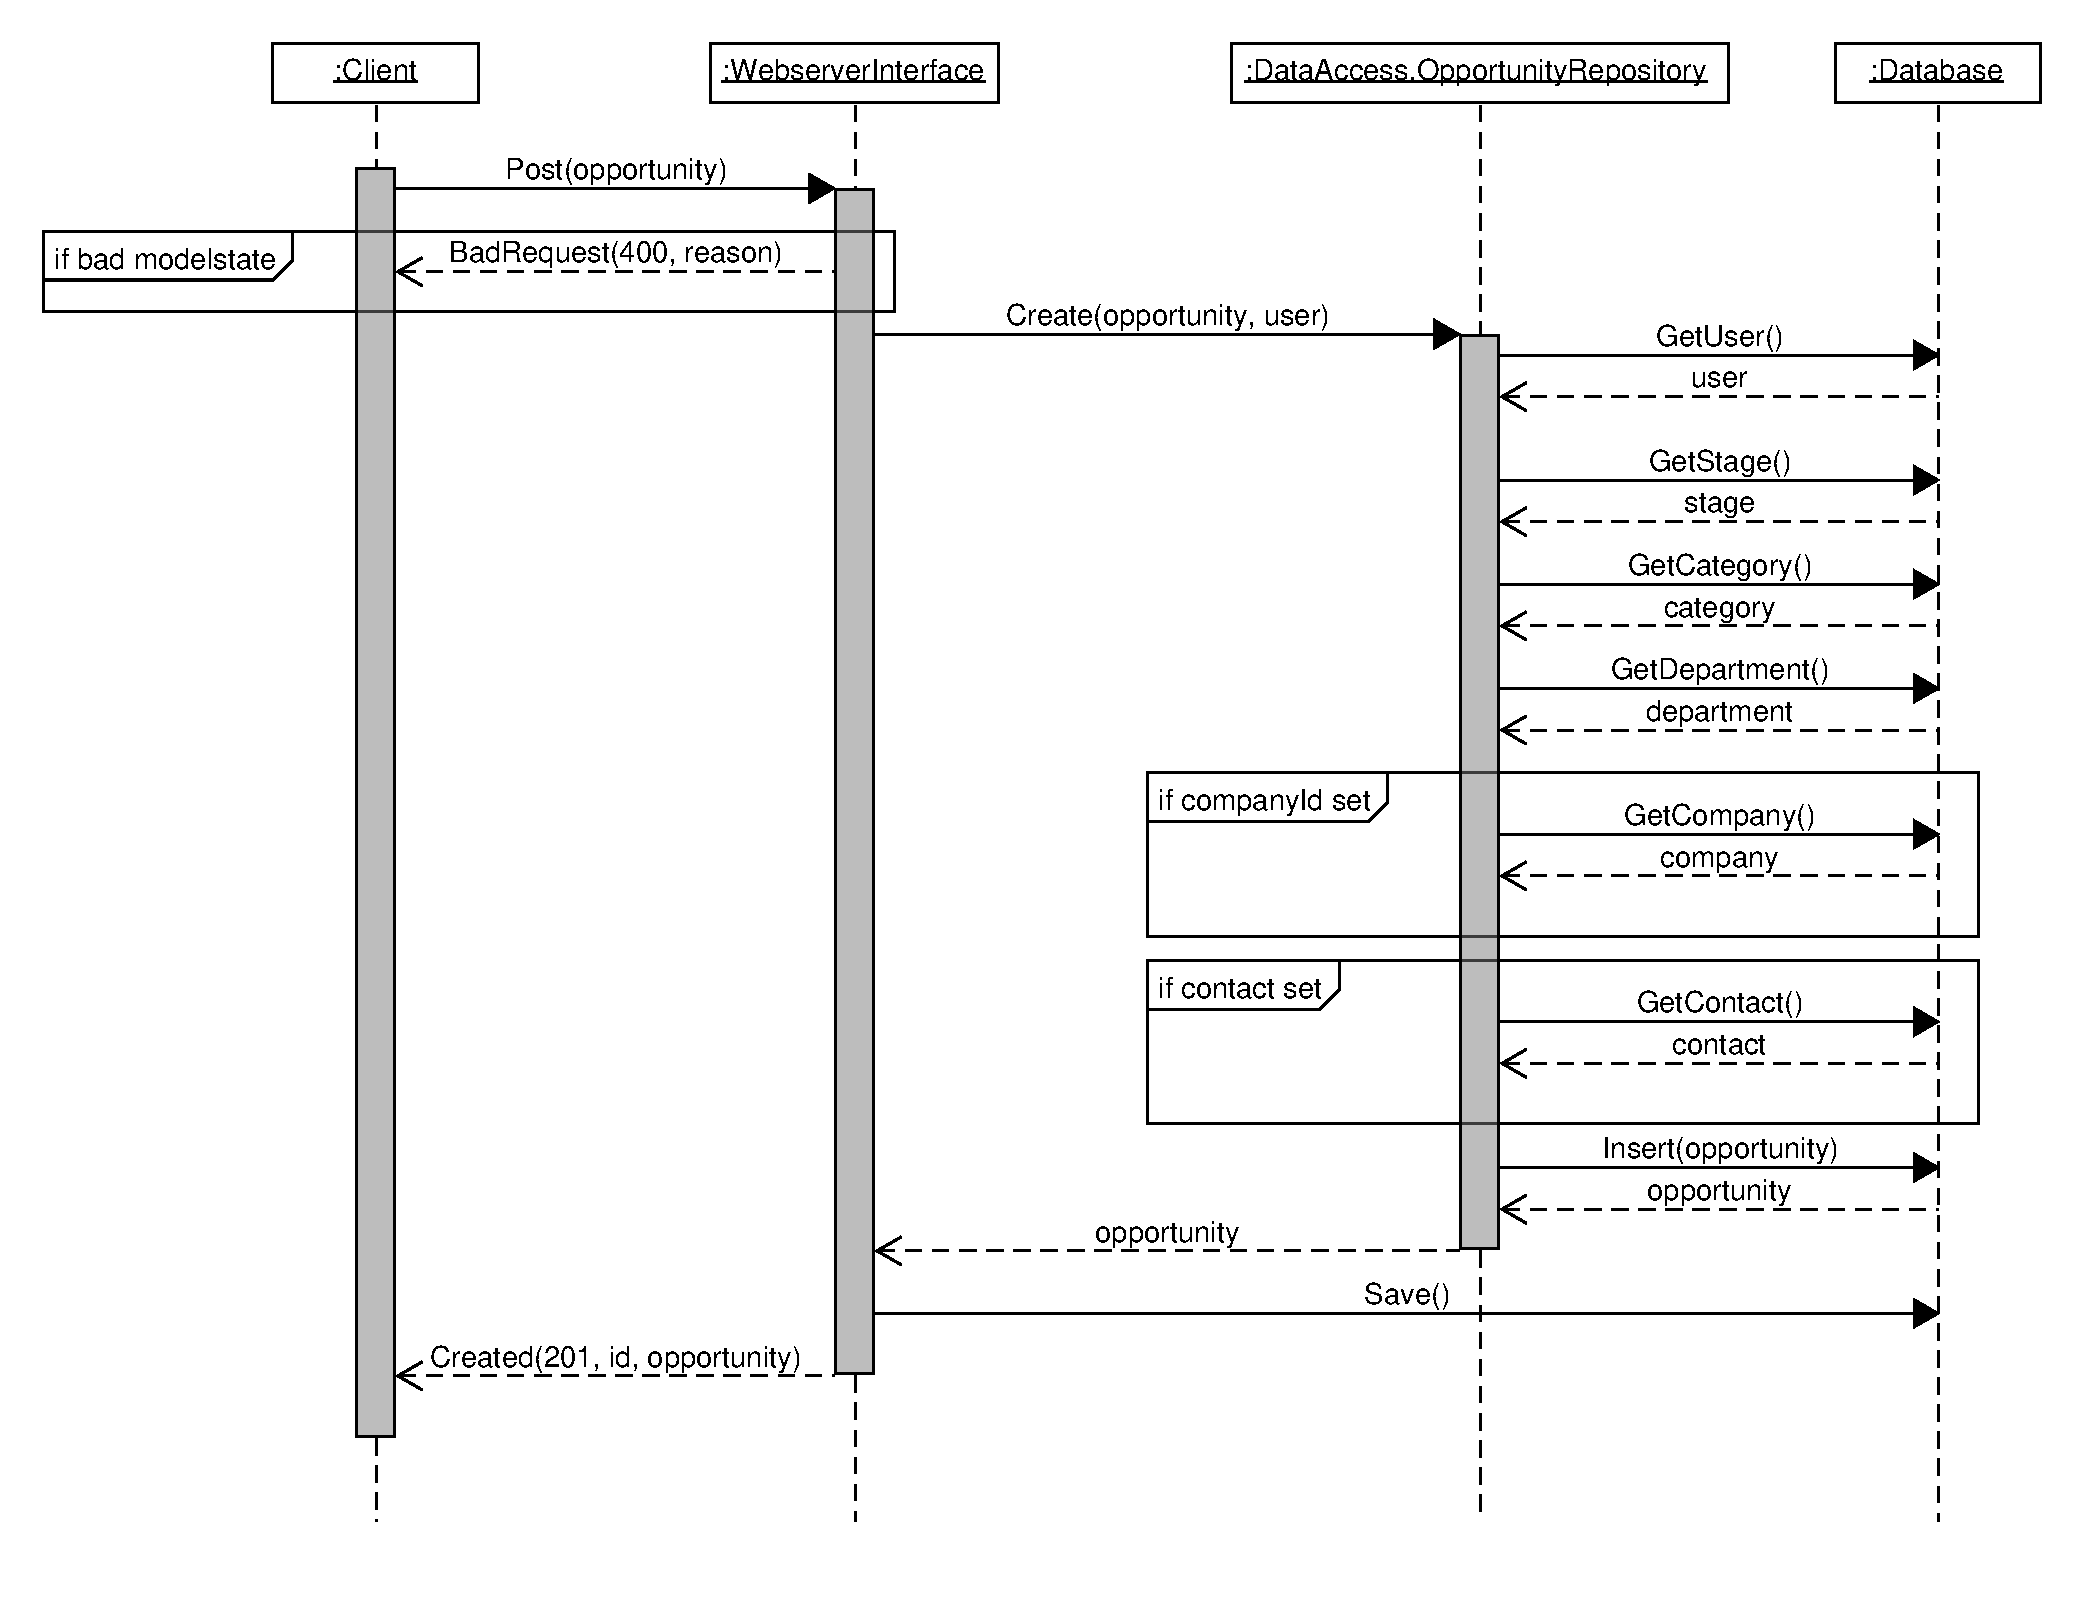
\includegraphics[width=\textwidth]{create_opportunity_sequence}
  \caption{Sequence diagram for creating a new opportunity}
  \label{fig:opportunity_sequence}
\end{figure}

I have not described the error possibilities in the creation of the opportunity,
as that would make the diagram harder to read, but for the required fields if we
turn out not to be able to find the element in the database we return a NotFound
to the client, which has the error code of 404. The return will be done by
throwing an exception in the place where we were supposed to find it, and let a
filter catch the error.

\section{Patterns}
\label{sec:Patterns}

\subsection{Dependency injection}
\label{sub:dependency_injection}
In order to reduce coupling in the code I use dependency injection.
Dependency injection is the idea of letting the caller instantiate all of our
dependencies instead of creating them in the class where I need it. 

There are several advantages of this, one of which is that I can easily isolate
a single unit of the program for testing, and then do unit testing on that
single unit. I can then make mocks of all of its dependencies, and therefore
know exactly how the different dependencies will react depending on my test
code\cite{dependency_injection}. 

A way to reduce coupling even further is to instead of depending on a specific
class. I can depend on an interface, which will allow me to only rely on a
specific set of methods of the class, and then the developer can decide what
implementation they find best suited. 

\subsection{Repository pattern}
\label{sub:repository_pattern}
The objective with the repository pattern is to separate the business logic away
from the data access logic, resulting in the business logic not caring about
where the data comes from, as it will just call a repository, and expect some
data to come back. 

An advantage of this pattern is that the developer implementing the business
logic can have a mocked implementation of the repository, that just uses some
form of local storage. It allows the developers to delay the decision of where
to store the data, as the repository does not have to be implemented to access a
database, but it could read from a file, request a web service, or something
else\cite{repository_pattern}. It also allows for easier swapping of storage
service, since the business logic would not have to be updated at all. 

\subsection{Unit of work pattern}
\label{sub:unit_of_work_pattern}
A pattern that works well with the repository pattern, that is described in
section~\ref{sub:repository_pattern}, is the unit of work pattern. The goal of
this pattern is to group up execution of operations that has an impact on the
data store. In cases where I just read out from the database I may not need it,
but in cases where I change data it makes sense to be in a state where I either
do all of the intended operations or none of them. 

The problem that the unit of work pattern solves is that if I am updating some
object, which includes the deletion of some data, I want to make sure that if
something fails later on after I have done the delete, so that the creation was
not done, the delete operation is abandoned, and I have not damaged my data
model\cite{uow}. 

\section{Class diagram}
\label{sec:class_diagram}

I have created class diagrams to help get an overview of how the different
classes are connected, one for each project. In
figure~\ref{fig:main_class_diagram} a diagram for the project containing the
controllers is represented, and in appendix~\ref{app:class_diagrams} the rest
are illustrated.

In figure~\ref{fig:main_class_diagram} it can be seen that the references to
repositories are done via interfaces, and are injected to lower the coupling
as described in section~\ref{sub:dependency_injection}.

It can also be seen that I use the repository pattern since the most common
dependency is a repository, along with a unit of work class, which allows me to
only know the repository, and how to save, as described in sections
\ref{sub:repository_pattern} and \ref{sub:unit_of_work_pattern}.

\doublepagepdf{class_diagrams/main_class_diagram}{Class diagram of
  customer\_relation\_manager}{fig:main_class_diagram} 

\section{Chapter summary}
The structure of the system is following the onion model, working around the
idea of layers, with the domain model as the inner core, which is the database
containing the data. The next layer is the domain services, describing how to
get the data from the database, followed by the application services, which is
in charge of doing data manipulation, and tasks that is essential to the system,
without dealing with a user yet. After this we have the implementation of the
data access, and the user interface, which will be the controllers, and the
served webpage.

From the use cases I have made a couple of sequence diagrams, describing the flow
from requesting client to the database and back, resulting in the client
getting the data that they request. 

In general I have designed the system to follow a principle of allowing the
repositories to throw exceptions if something goes wrong. These exceptions are
then caught and transformed into proper responses based on the exception thrown.

I follow a couple of patterns in the development. Some of them are dependency
injection, which allows me to lower the coupling in the system, and allows me
to make unit tests easier, since i can control all the dependencies of a class
at the time of instantiation.

I use the repository pattern to separate the accessing of data away from the
controllers, as they are not meant to deal with the actual implementation of
that, but rather make sure that the communication is correct, and the right
tasks are done.

Another pattern I use is the Unit of Work pattern which makes sure that my data
never ends up in an unknown state because something failed half way through an
operation, but only if I make it all the way through the changes are saved.

To illustrate some of the pattern uses, and to give a better idea of the
structure of the system I have created some class diagrams. The the primary one,
which illustrates the controllers, and their relations, and types is illustrated
in figure~\ref{fig:main_class_diagram}, while the rest are in
appendix~\ref{app:class_diagrams}.